\documentclass[10pt,a4paper]{article}
\usepackage[latin1]{inputenc}
\usepackage{amsmath}
\usepackage{amsfonts}
\usepackage{amssymb}
\usepackage{graphicx}
\author{Carter Rhea}
\title{Phys 760: PS 1 Solutions}
\begin{document}
	\maketitle
	\section{Problem 1}
	\textbf{Explain why a positive definite inner product is non-degenerate}\\
	Proof: Assume we have a positive definite inner product ($\cdot$,$\cdot$). Then given some function $g$ we have $(g,g) = 0 \Leftrightarrow g = 0$.\\
	Claim: Given any function $f$ such that $(f,g) = 0$, then $g=0$.\\
	By Contradiction: Assume $g \neq 0$. Then there exists some $f$ such that $f=g$ where $(f,g)=0$ and $g\neq0$ which contradicts the definition of a positive definite inner product. Therefore $g=0$, as required.
	
	\section{Problem 2}
	\textbf{Show that a non-negative inner product with the property that $(f,f)=0$ implies that $\forall g (g,f) = 0$}\\
	Proof: Assume we have a non-negative inner product ($\forall f (f,f) \geq 0$).\\
	Claim: $(f,f)=0 \rightarrow \forall g (g,f)=0$\\
	By Contradiction: Assume $\exists g s.t. (g,f)\neq 0$. However, if we allow $f=g$ then by the definition of a non-negative inner product $(g,f) = (g,g) = 0$ which is a contradiction to the initial assumption. Therefore $\forall g (g,f)=0$.
	
	\section{Problem 3}
	\textbf{Show that if a linear operator is represented by a hermitian matrix in an orthonormal basis, then $(g,Af)=(Ag,f)$}.\\
	Proof: Assume we have a linear operator $A$ such that $A$ is a hermitian matrix ($A=A^\dagger$) in an orthonormal bases ($A*A^T=0$). Then we have the following:

		$$(g,Af) = (g,A^\dagger f) = (Ag,AA^\dagger f) = (Ag,f)$$

	\section{Problem 4}
	\textbf{Show The Epsilon-Delta Correspondence}\\
	Claim: 
	$$\sum_{i=1}^3 \epsilon_{ijk}\epsilon_{inm} = \delta_{jn}\delta_{km}-\delta_{jm}\delta_{kn}  $$
	$$
		\sum_{i=1}^3 \epsilon_{ijk}\epsilon_{inm} = \epsilon_{1jk}\epsilon_{1nm} + \epsilon_{2jk}\epsilon_{2nm} + \epsilon_{3jk}\epsilon_{3nm}
		=  \left\{
		\begin{array}{ll}
		1 & j=n \ \& \ k=m\\
		-1 & j=m \ \& \ k=n \\
		0 & else \\
		\end{array} 
		\right.
	$$
	$$
	\delta_{jn}\delta_{km}-\delta_{jm}\delta_{kn}
	=  \left\{
	\begin{array}{ll}
	1 & j=n \ \& \ k=m\\
	-1 & j=m \ \& \ k=n \\
	0 & else \\
	\end{array} 
	\right.
	$$

	\section{Problem 5}
	\subsection{Part A}
	\textbf{Non-singular $NxN$ matrices form a vector space of dimension $N^2$}\\
	This is false because the $0$ matrix is singular and thus not a part of the set created from non-singular matrices.
	\subsection{Part B}
	\textbf{Singular $NxN$ matrices form a vector space of dimension $N^2$}\\
	 False. The addition of two singular matrices is not always singular!
	 \begin{equation}
	 	\begin{bmatrix}
		 	1 & 0\\
		 	0 & 0
	 	\end{bmatrix}
	 	+
	 	\begin{bmatrix}
		 	0 & 0\\
		 	0 & 1
	 	\end{bmatrix}
	 	=
	 	\begin{bmatrix}
		 	1 & 0 \\
		 	0 & 1
	 	\end{bmatrix}
	 \end{equation}

	\subsection{Part C}
	\textbf{Complex numbers form a vector space of dimension 2}\\
	True!! It is very easily shown that the addition of two complex numbers is a complex number, the scalar multiplication of a complex number is still complex, and the number $0$ is a complex number (albeit a very boring one!).
	
	\subsection{Part D}
	\textbf{Polynomial functions of $x$ form an infinite-dimensional vector space}\\
	True
	
	\subsection{Part e}
	\textbf{Series $\{a_0,a_1,\dots ,a_N\}$ for which $\sum_{n=0}^N|a_n|^2 = 1$ form an $N-dimensional$ vector space.}\\
	False. It is simply not possible to have the zero vector (or zero series) satisfying the summation.




	\section{Problem 6}
	\subsection{Part A}
	\textbf{If A is Hermitian and U is unitary then $U^{-1}AU$ is Hermitian} \\
	Proof: Assume $A$ is Hermitian and $U$ is unitary. Then we have the following properties:
	$$A = A^\dagger $$
	$$UU^\dagger = I \Rightarrow U=U^{-\dagger} \Rightarrow U^{-1} = U^\dagger $$
	
	Hence we can do the following...
	
	\begin{equation}
		\begin{split}
			U^{-1}AU & = \sum_{jk} u^{-1}_{ij}a_{jk}u{kl}\\
			& = u_{ji}^\star a_{kl}^\star u_{kl} \ \ (\text{by properties above})\\
			& = u_{ji}^\star a_{kj}^\star u_{lk}^{-\star} \ \ (\text{by properties above})\\
			& = (UAU^{-1})^\star \\
			& = (U^{-1}AU)^\dagger
		\end{split} 
	\end{equation}
	Therefore $$U^{-1}AU = (U^{-1}AU)^\dagger $$
	
	\subsection{Part B}
	\textbf{If A is antiHermitian then $i$A is Hermitian}\\
	Note: Definition of antiHermitian $:= a_{ij}=-a_{ji}^\star$.\\
	Let $a_{ij} = c+di$. By definition of skew-hermitian we have, $a_{ij}=-a{ji}^\star$.
	
	\begin{equation}
		\nonumber
		\begin{split}
			a_{ji}=c+di&\rightarrow -a_{ji}^\star = c+di\\
			&\rightarrow a_{ji}^\star = -c-di\\
			&\rightarrow a_{ji} = -c+di
		\end{split}
	\end{equation}
	Let now $B=iA \leftarrow b_{ij} = ci-d$
	Hence we have :
	\begin{equation}
		\begin{split}
			b_{ij} = ci-d & \rightarrow b_{ji} = ci-d \ \ (\text{from definition of } a_{ji})\\
			& \rightarrow b_{ji}^\star = ci-d
		\end{split}	
	\end{equation}
	
	Therefore $B=iA$ is Hermitian!
	
	\subsection{Part C}
	\textbf{The product of two Hermitian matrices A and B is Hermitian iff A and B commute}\\
	($\Rightarrow$) Assume the product of two matrices Hermitian matrices is Hermitian. \\
	By Contradiction: Assume $AB\neq BA$. By definition of Hermitian we have:
	$$\sum_{k=1}^{N}a_{ik}b_{kj}  = AB = (AB)^{\dagger} = \Big(\sum_k a_{ik}b_{kj}  \Big)^\dagger  = \Big(\sum_k a_{ik}^\star b_{kj}^\star  \Big)^T = \Big( \sum_k b^\star_{jk}a^\star_{ki} \Big)$$
	However we must note that 
	\begin{equation}
	\nonumber
		\begin{split}
		a_{ik}b_{kj} &\neq b_{kj}a_{ik}  \ \  (\text{by definition of non-commuting})\\
		& = b^\star_{jk}a^\star_{ik} \ \ (\text{by definition of Hermitian})
		\end{split}
	\end{equation}
	Hence we have a contradiction
	\\
	($\Leftarrow$) Assume $AB=BA$ and $A,B$ are Hermitian matrices. \\
	By Contradiction: Assume $AB \neq (AB)^\dagger$. Hence, $$\sum_k a_{ik}b_{kj} \neq b_{jk}^\star a_{ki}^\star $$
	But since $A$ and $B$ are Hermitian we know,
	 $$a_{ij}=a_{ji}^\star  \ \& \  b_{ij}=b_{ji}^\star $$
	Furthermore, since $AB=BA$ we can pick an arbitrary element such that we have,
	\begin{equation}
	\begin{split}
		\sum_k a_{ij}b_{jk} & = b_{kj}a_{ji} \ \ \text{by definition of commutative}\\
		& = b_{jk}^\star a{_ij}^\star \ \ \text{since $A$ and $B$ are Hermitian} 
	\end{split}
	\end{equation}
	However this is a contradiction. Therefore $AB$ must be Hermitian!
	
	\subsection{Part D}
	\textbf{If S is a real antisymmetric matrix then $A=(!-S)(1+S)^{-1}$ is orthogonal}\\
	Note that $S^T = -S$ by definition of antisymmetric.
	\begin{equation}
	\nonumber
		\begin{split}
			A^TA &= (1+S)^{-T}(1-S)^{T}(1-S)(1+S)^{-1}\\
			&= (1+S)^{-T}(1-S^T)(1-S)(1+S)^{-1}\\
			&= (1+S)^{-T}(1+S)(1-S)(1+S)^{-1}\\
			&= (1-S)^{-1}(1-S^2)(1+S)^{-1}\\
			&= (1-S)^{-1}(1-S)(1+S)(1+S)^{-1}\\
			&= I * I\\
			&= I 
		\end{split}
	\end{equation}
	
	
	\subsection{Part E}
	\textbf{If $K$ is antihermitian, then $V=(1+K)(1-K)^{-1}$ is unitary}\\
	Note $K^\dagger = -K$. Claim: $V^\dagger V=1$
	\begin{equation}
	\nonumber
		\begin{split}
			VV^\dagger &= (1+K)(1-K)^{-1}(1-K^\dagger)^{-1}(1+K^\dagger)\\
			&= (1-K^\dagger)(1+K^\dagger)^{-1}(1-K^\dagger)^{-1}(1+K^\dagger)\\
			&= I*I\\
			&= I
		\end{split}
	\end{equation}
	
	
	
	\section{Problem 7}
	\textbf{Two anticommuting matrices $A$ and $B$ satisfy $AB+BA=0$. If $A^@=B^2=1$ and $[A,B]=2iC$}
	\subsection{Prove $C^2=1$ and that $[B,C]=2iA$}
	\begin{equation}
	\nonumber
		\begin{split}
			(AB-BA)^2 &= (2iC)^2\\
			ABAB-ABBA-BAAB-BABA &= -4C^2\\
			-1 -ABBA - BAAB -1 &=  -4C^2 \ | \ \text{ABAB = BABA = -1 through the anticommuting property}\\
			-1 -1 -1 -1 &= -4C^2\\
			1 &= C^2
		\end{split}
	\end{equation}
	

	
	\begin{equation}
	\nonumber
		\begin{split}
			[B,C] &= BC-CB \\
			& = B(\frac{AB-BA}{2i})-\frac{AB-BA}{2i}B \\
			& = \frac{BAB-BBA}{2i} - \frac{ABB-BAB}{2i}\\
			&= \frac{1}{2i}(BAB-BBA-ABB+BAB)\\
			&= \frac{1}{2i}(-BBA-BBA-BBA-BBA)\\
			&= \frac{-4BBA}{2i}\\
			&= 2iA
		\end{split}
	\end{equation}
	
	
	\subsection{Evaluate $[[[A,B],[B,C]],[A,B]]$}
	\begin{equation}
		\nonumber
		\begin{split}
			[[[A,B],[B,C]],[A,B]] &= [[2iC,2iA],[2iC]]\\
			&= [-4CA-4AC,2ic]\\
			&= -8iCAC-8iACC-8iCCA-8iCAC\\
			&= -16iA-16iCAC\\
			&= -32iA
		\end{split}
	\end{equation}
	
	\section{Problem 8}
	\textbf{Show $x=(A^\dagger A)^{-1}A^\dagger y$ is the  minimization for our error norm $E$}\\
	Let $E'=M*E^2$ for our sanity. Note that now we can define $E'$ in the following manner:
	$$E' = (y-Ax)^\dagger(y-Ax) = (y^\dagger -A^\dagger x^\dagger)(y-Ax) = (y^\dagger y - A^\dagger x^\dagger y - y^\dagger Ax + A^\dagger x^\dagger Ax) $$
	Now our main goal will be the common minimization technique of taking the derivative and setting it equal to zero...
	\begin{equation}
	\nonumber
	\begin{split}
		\frac{dE'}{dx} &= \frac{d}{dx}\Big\{  y^\dagger y - A^\dagger x^\dagger y - y^\dagger Ax + A^\dagger x^\dagger Ax \Big\}
		= -y^\dagger A - y^\dagger A+2x^\dagger A^\dagger A\\
	\end{split}
	\end{equation}
	
	$$y^\dagger A = x^\dagger A^\dagger A $$
	$$x^\dagger = y^\dagger A(A^\dagger A)^{-1} $$
	$$x = (y^\dagger A(A^{-1}A^{-1}))^\dagger = (A^\dagger A)^{-1}A^\dagger y  $$
	
	
	
	\section{Problem 9}
	\textbf{Find the SVD for our matrix...}
	Using python this is trivial...\\
	$numpy.linalg.svd(np.matrix([[0,-1],[1,1],[-1,0]]))$ returns the following:
	
	\begin{figure}
		\centering
			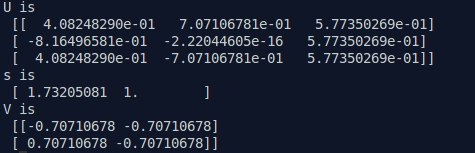
\includegraphics[width=0.8\textwidth]{svd}
	\end{figure}

	\section{Problem 10}
	I found all of the problems were quite reasonable and a good portion of my time was spend typing everything up!
	
	
	
	
	
	
	
	
	
	
	
	
\end{document}